\chapter{Generadores de Números Aleatorios}

%%%%%%%%%%%%%%%%%%%%%%%%%%%%%%%%%%%%%%%%%%%%%%%%%%%%%%%%%%%%%%%%%%%%%%%%%%%%%
\section{Cripto-Codificación caótica Variante en el tiempo}

\subsection{Introdución}

En los sistemas de comunicaciones y particularmente en los
dedicados a la codificación para el control de error y
encriptamiento de datos se usan técnicas derivadas de la teoría de
señales. Estas técnicas se aplican típicamente en la forma lineal
debido a la simplicidad que ésto trae aparejado. Además cada una se
implementa algorítmicamente o físicamente como una entidad
independiente. Para cada sistema en particular se las elige
con criterios de conveniencia práctica, y se las aplica en forma
consecutiva o encadenada. La teoría de los sistemas no lineales
\cite{Strogatz1994,Lasota1994} aparece como un marco de trabajo
ideal para ser utilizado en el contexto anteriormente mencionado.
La existencia de los sistemas caóticos, y la relación de estos con
la aleatoriedad, o pseudo aleatoriedad, otorga una plataforma de
diseño que hasta hoy se encuentra poco explotada.

En los últimos veinte años se han presentado diversos trabajos que
emplean caos en los sistemas de comunicaciones, como por ejemplo
el empleo de portadoras caóticas sincronizadas en las
transmisiones analógicas \cite{Kocarev1995,Hidalgo2001}. Si nos
centramos en la representación discreta un referente muy
importante es el excelente trabajo de Kozic et. als.
\cite{Kozic2006A,Kozic2006B} en el que se presenta una técnica de
modulación empleando mapas caóticos unidimensionales lineales por
tramos, la técnica consiste en la introduccíón del mensaje a
codificar en el bit menos significativo de la secuencia generada.
Obteniéndose una secuencia levemente alterada lo que impide que el
sistema entre en ciclos periódicos.

En este trabajo se propone un grupo de atractores como generadores de señales
pseudoaleatorias para realizar el proceso de codificación y
encriptamiento. El esquema de codificación se basa
en una familia de mapas cuadráticos bidimensionales, cuyas salidas
presentan comportamiento caótico, con distintos atractores
conforme a los coeficientes que se empleen. La idea es que cada
palabra a codificar sea unívoca con un juego de coeficientes que
serán parámetros de un mapa cuadrático bidimensional. Como
resultado de este procedimiento, la señal de salida son puntos
pertenecientes a distintos atractores elegidos por la información
a transmitir.

La ventaja de este método reside en que la
estructura de toda la familia de mapas es única y común, modificándose
solamente los coeficientes se consiguen atractores distintos. Esta
priopiedad reduce y facilita la implementación en hardware.
Resultados preliminares obtenidos mediante simulaciones muestran
que el sistema presenta una performance comparable a la
obtenida en sistemas clásicos de encriptamiento, en cuanto a
probabilidad de error y a distancia mínima.


\subsection{Mapas cuadráticos bidimensionales}


En este trabajo se emplea una familia de mapas cuadráticos
bidimensionales cuya estructura consta de dos ecuaciones
cuadráticas en diferencias acopladas (Ec.\ref{eq:Qmap}). La
característica principal de este mapa es que los parámetros, $a_i$
y $b_i$, son coeficientes reales y para ciertos valores de estos
coeficientes la salida del sistema presentará comportamiento
caótico.

Se obtiene así un subgrupo de mapas distintos con comportamiento
caótico según la elección de estos coeficientes, en la Fig.
\ref{fig:atractores} puede verse tres atractores para tres juegos
distintos de valores de los coeficientes.

Estos mapas han sido ampliamente estudiados, por lo que la
estabilidad, la sensibilidad a las condiciones iniciales y su
dimensión fractal son parámetros ya conocidos
\cite{Sprott2003,Sprott2000}.

\begin{eqnarray}\label{eq:Qmap}
    x_{n+1}&=& a_0 + a_1 x_n + a_2 x_n^2 + a_3 x_n y_n + a_4 y_n^2 + a_5 y_n \nonumber\\
    y_{n+1}&=& b_0 + b_1 x_n + b_2 x_n^2 + b_3 x_n y_n + b_4 y_n^2 + b_5 y_n
\end{eqnarray}

%hablar sobre mapas perturbados por la información
\begin{figure}
    \centering
    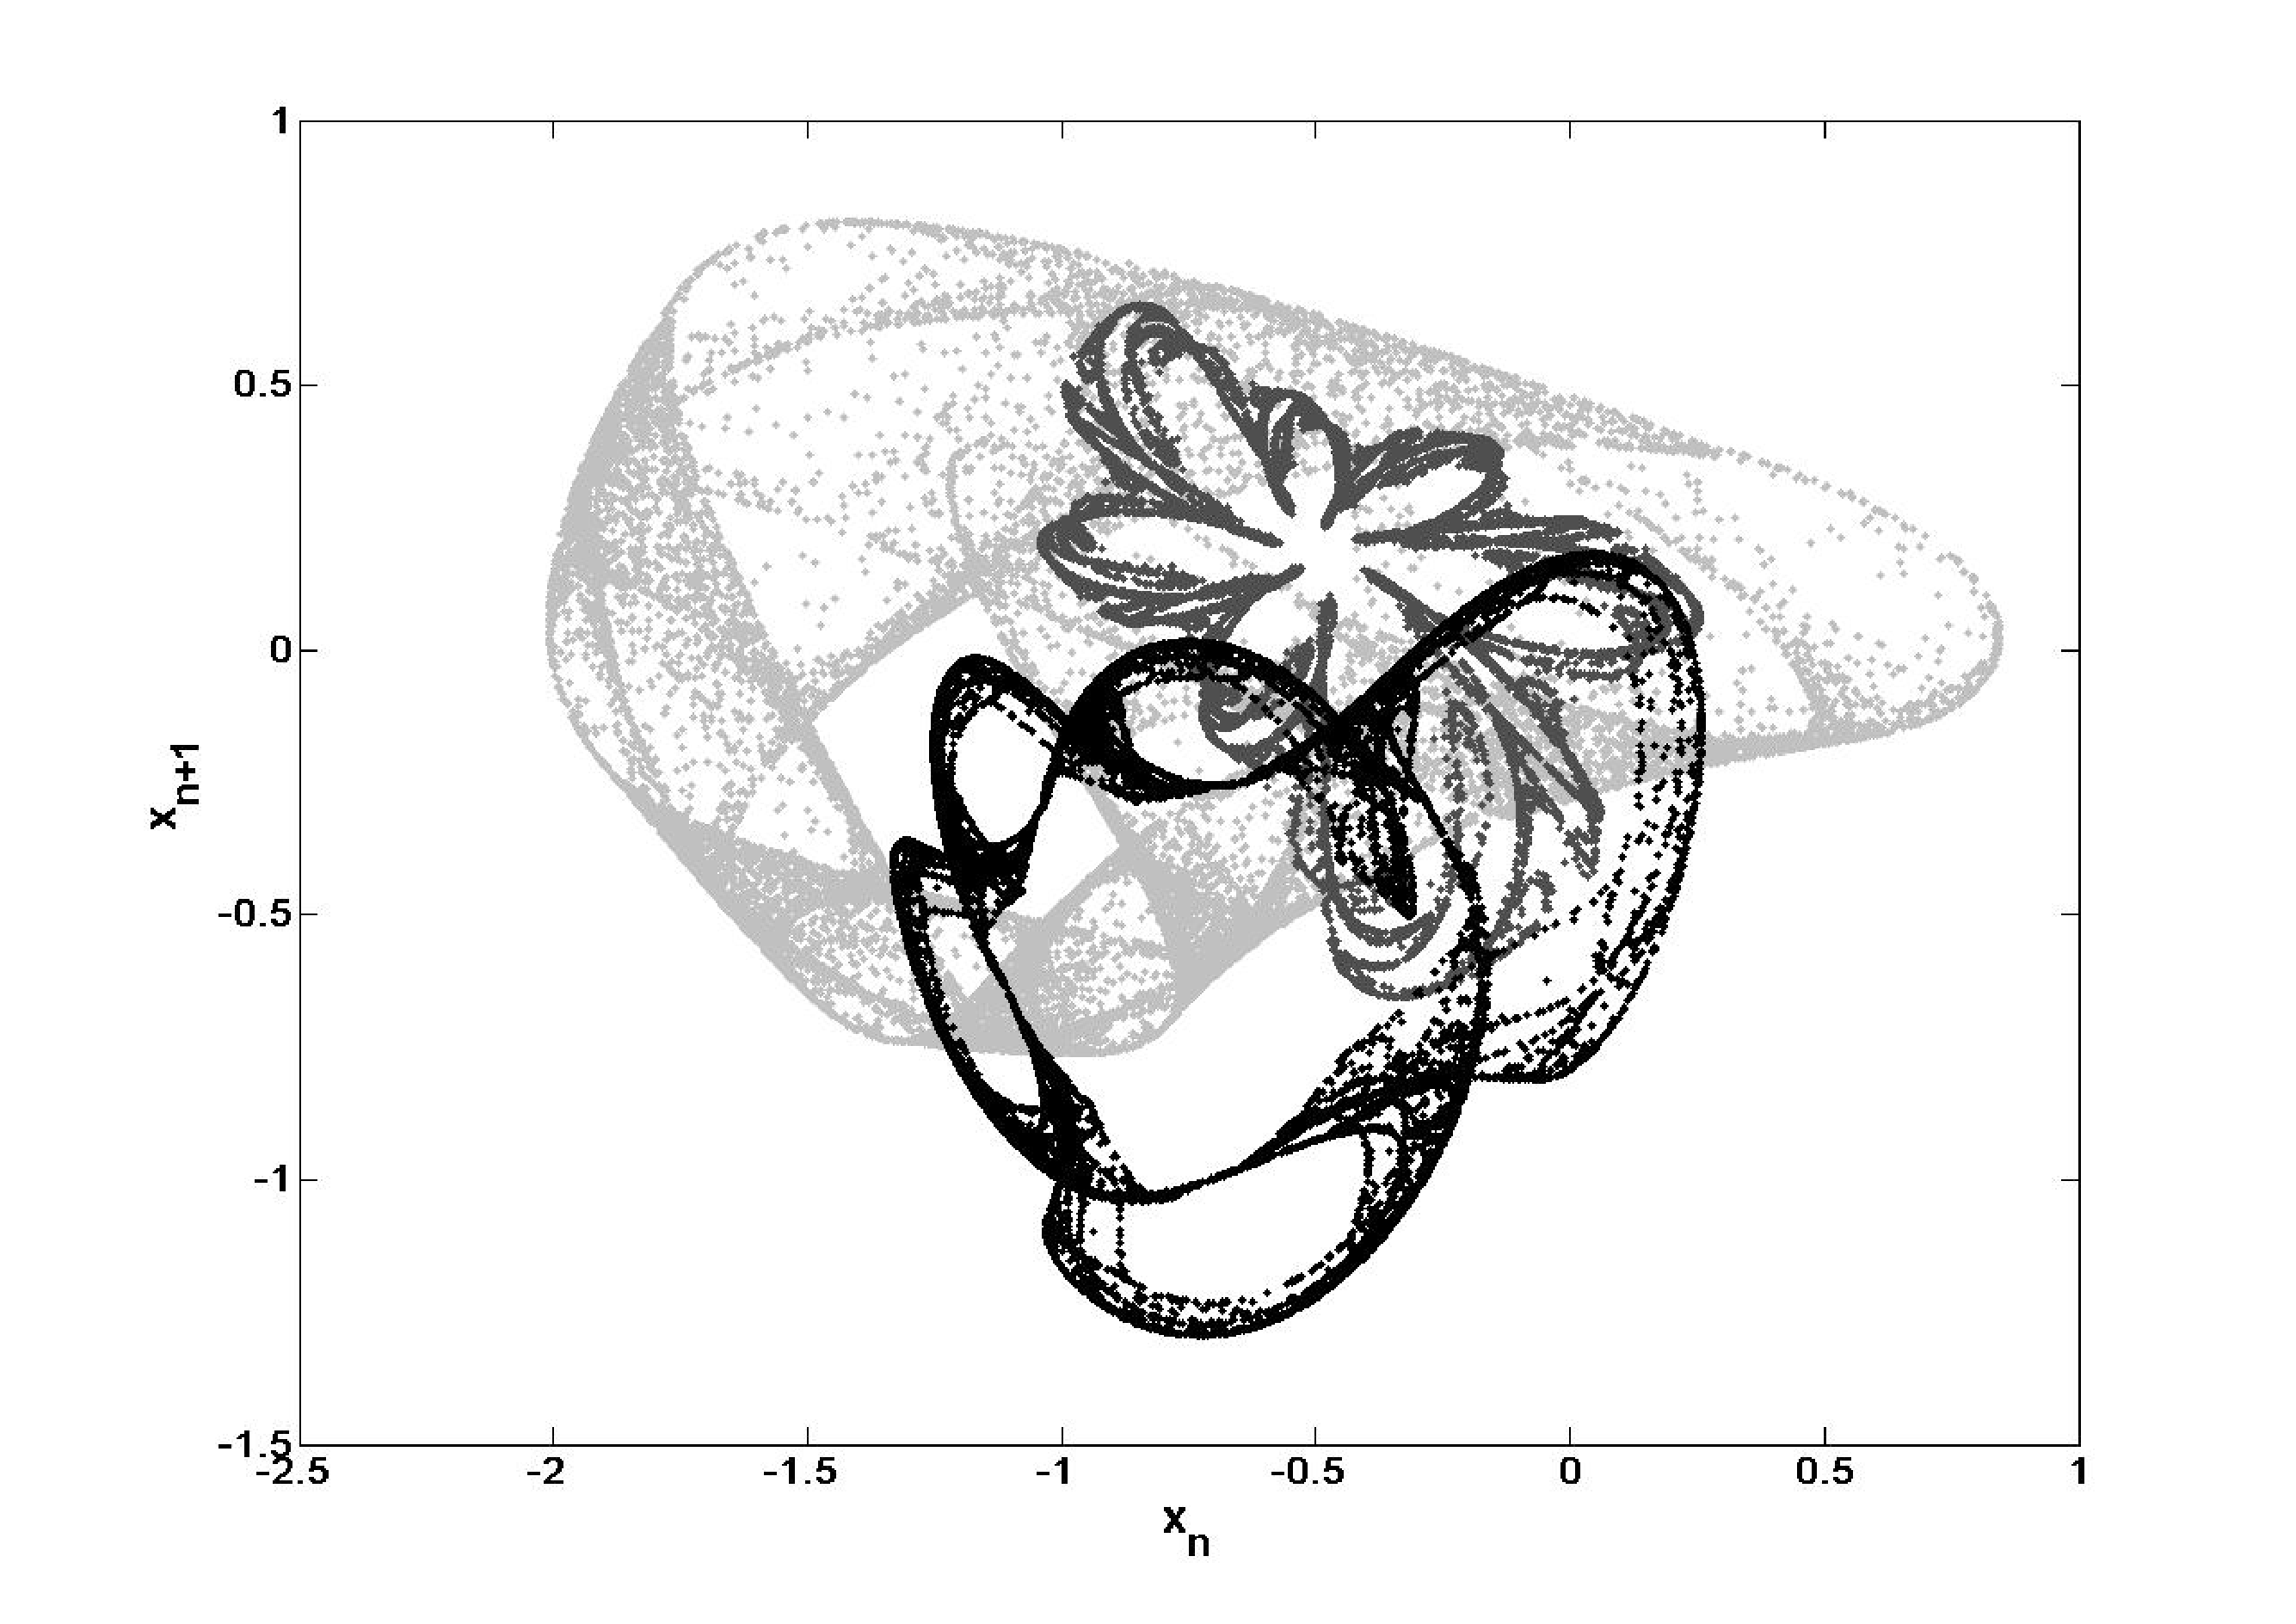
\includegraphics[width=1\columnwidth]{atractores.pdf}\\
    \caption{Atractores del sistema para tres juegos de coeficientes.}\label{fig:atractores}
\end{figure}

\subsection{Implementación}

Desde el punto de vista del esquema de codificación propuesto,
estos mapas son muy atractivos por el hecho de contar con $12$
coeficientes para generar cada atractor. Por lo tanto, las
combinaciones posibles serán $N^{12}$, en donde $N$ es la cantidad
de símblos posibles según la aritmética utilizada. En nuestro caso
empleamos una aritmética de $19$ bits expresados en complemento a
$2$ con aritmética de punto fijo, con $1$ bit de signo, $3$ bits
de parte entera y $15$ bits de parte decimal. Esta aritmética
limita y discretiza el plano $xy$ que queda delimitado por $\Delta
x=4$, $-\Delta x=-4$, $\Delta y=4$,$-\Delta y=-4$, como puede
verse en la figura \ref{fig:atractores}. Estas limitaciones al
plano de atracción tienen como consecuencia dos cuestiones a tener
en cuenta:
\begin{itemize}
    \item
        Debido a que los coeficientes se generan con la misma aritmética que las variables, nos
        encontramos con $N=2^{19}$ valores posibles para cada coeficiente,
        lo que arroja $\left(2^{19}\right)^{12}\cong4,3^{68}$ combinaciones posibles de coeficientes para generar distintos atractores.
    \item
        En cuanto a las trayectorias de los atractores sobre el plano discretizado,
        éstas se tornan periódicas debido a la discretización.
\end{itemize}


No todos los juegos de coeficientes generan atractores caóticos contenidos en el plano dado por la aritmética utilizada. Aunque esto no sería problema para la codificación/decodificación, se eligieron los coeficientes de modo que se generen atractores contenidos en el plano a modo de validación visual.

Dada la naturaleza de los mapas caóticos, un punto muy lejano a la zona de atracción puede hacer que el punto calculado para la próxima iteración diverja, por lo tanto las condiciones iniciales deben ser normalizadas antes de cambiar al mapa siguiente. Para solucionar este problema se utiliza la siguiente estrategia:
 Primero se define el plano mínimo que contiene al atractor. Para
        identificarlo se simularon los mapas mediante Quartus
        generando secuencias de salida lo suficientemente largas como para
        verificar la periodicidad. Luego se analizó este vector de datos
        con Matlab buscando los valores extremos en cada una de las
        variables: $X1_{max}$, $X1_{min}$, $Y1_{max}$, $Y1_{min}$. Estos límites delimitan al plano mínimo que contiene al atractor. La normalización dada por la ecuación \ref{eq:norm_salida} se aplica a la salida $\left(x,y\right)$ para mapear este plano minimo a todo el plano delimitado por la aritmética utilizada de dimensiones $\Delta x$, $-\Delta x$, $\Delta y$, $-\Delta y$.
Segundo, se halla el plano máximo que contiene las condiciones
iniciales que hacen que no diverja la solución sinó que genere el
atractor. Para esto se realizó un programa en Matlab que genera
los atractores desde todas las condiciones iniciales del plano
delimitado y discretizado por la aritmética utilizada, a
continuación se marcan todos los puntos que generan trayectorias
divergantes o bien convergentes a un punto fijo. Este proceso
genera la zona de condiciones iniciales factible para generar
atractores, nuevamente se identificaron los valores máximos y
mínimos del área rectangular máxima que contenga todos sus puntos
como condiciones iniciales factibles $X2_{max}$, $X2_{min}$,
$Y2_{max}$, $Y2_{min}$. La normalización dada por la ecuación
\ref{eq:norm_entrada} se aplica a la entrada de condiciones
iniciales $\left(x_{n-1},y_{n-1}\right)$ para mapear todo el plano
de dimensiones $\Delta x$, $-\Delta x$, $\Delta y$ y $-\Delta y$
al de condiciones iniciales factibles.


El problema de la existencia de puntos fijos para cierto conjunto de
coeficientes y condiciones iniciales queda salvado al perturbar
continuamente al atractor actual con valores afectados por la
información.

Se generó un circuito en VHDL con un total de $16$ juegos de
parámetros seleccionables con la palabra de entrada de $4$ bits
que se desea encriptar. Esta palabra multiplexa estos coeficientes
y alimenta un oscilador que calcula la próxima iteración de datos,
además, este circuito almacena la salida del oscilador y la
realimenta como ``condición inicial" para calcular la iteración
siguiente (Fig. \ref{fig:generador}). Como resultado de este
proceso, la salida encriptada resulta ser el oscilador actual
seleccionado por la palabra de entrada perturbado por la historia
de los mapas seleccionados por las entradas anteriores. Este
circuito de dos bloques se encarga de generar los atractores, por
lo que se lo llama ``generador de atractores".


Para la primer iteración, las condiciones iniciales son $(x;y)=(0.1;0.1)$ para cualquiera de los atractores.



\begin{figure}
    \centering
    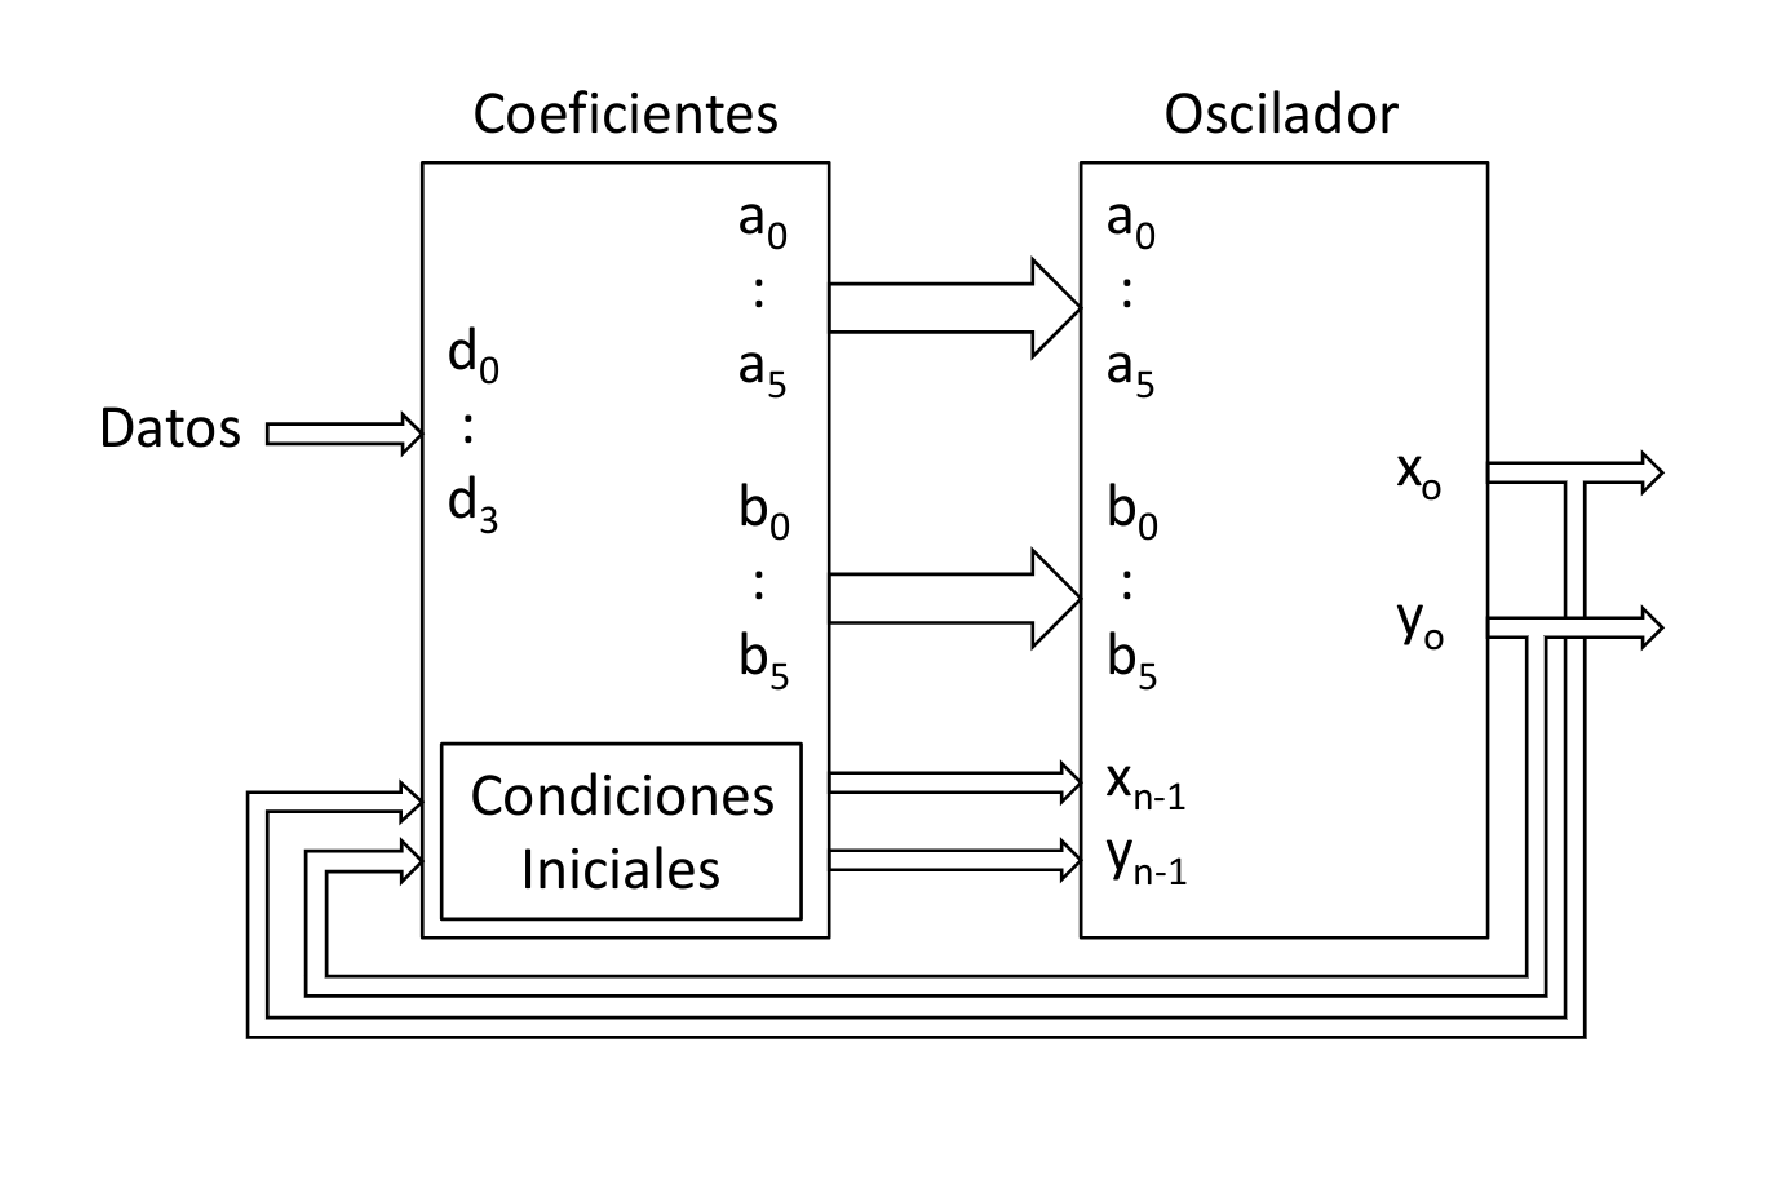
\includegraphics[width=0.7\columnwidth]{Fig1.pdf}\\
    \caption{Generador de atractores.}\label{fig:generador}
\end{figure}
{\small
\begin{eqnarray}\label{eq:norm_salida}
    x_{1norm}&=& a_{1x} x+b_{1x} \nonumber\\
    y_{1norm}&=& a_{1y} y+b_{1x} \nonumber\\
    a_{1x}&=& \frac{2\Delta x}{x1_{max}-x1_{min}} \nonumber\\
    a_{1y}&=& \frac{2\Delta y}{y1_{max}-y1_{min}} \nonumber\\
    b_{1x}&=& -\frac{x1_{max}-x1_{min}}{2} \nonumber\\
    b_{1x}&=& -\frac{y1_{max}-y1_{min}}{2}
\end{eqnarray}}
{\small
\begin{eqnarray}\label{eq:norm_entrada}
    x_{1norm}&=& a_{2x} x+b_{2x} \nonumber\\
    y_{1norm}&=& a_{2y} y+b_{2x} \nonumber\\
    a_{2x}&=& \frac{x2_{max}-x2_{min}}{2\Delta x} \nonumber\\
    a_{2y}&=& \frac{y2_{max}-y2_{min}}{2\Delta y} \nonumber\\
    b_{2x}&=& \frac{x2_{max}-x2_{min}}{2} \nonumber\\
    b_{2x}&=& \frac{y2_{max}-y2_{min}}{2}
\end{eqnarray}}

\subsubsection{Codificador}
El bloque del Codificador consiste en circuito generador y
acondicionamiento de la salida. Para codificar una palabra de
cuatro bits de entrada se generan los valores de $x$ e $y$ con el
circuito generador correspondiente a esta palabra y se los concatena en un circito posterior
formando un vector $[x:y]$ (Fig. \ref{fig:codificador}). De esta forma cada palabra de información a ser enviada será representada por la salida $xy$  del oscilador del atractor correspondiente, por lo tanto una palabra a codificar no se corresponderá con una palabra codificada, dos palabras iguales generarán dos salidas distintas.


\begin{figure}
    \centering
    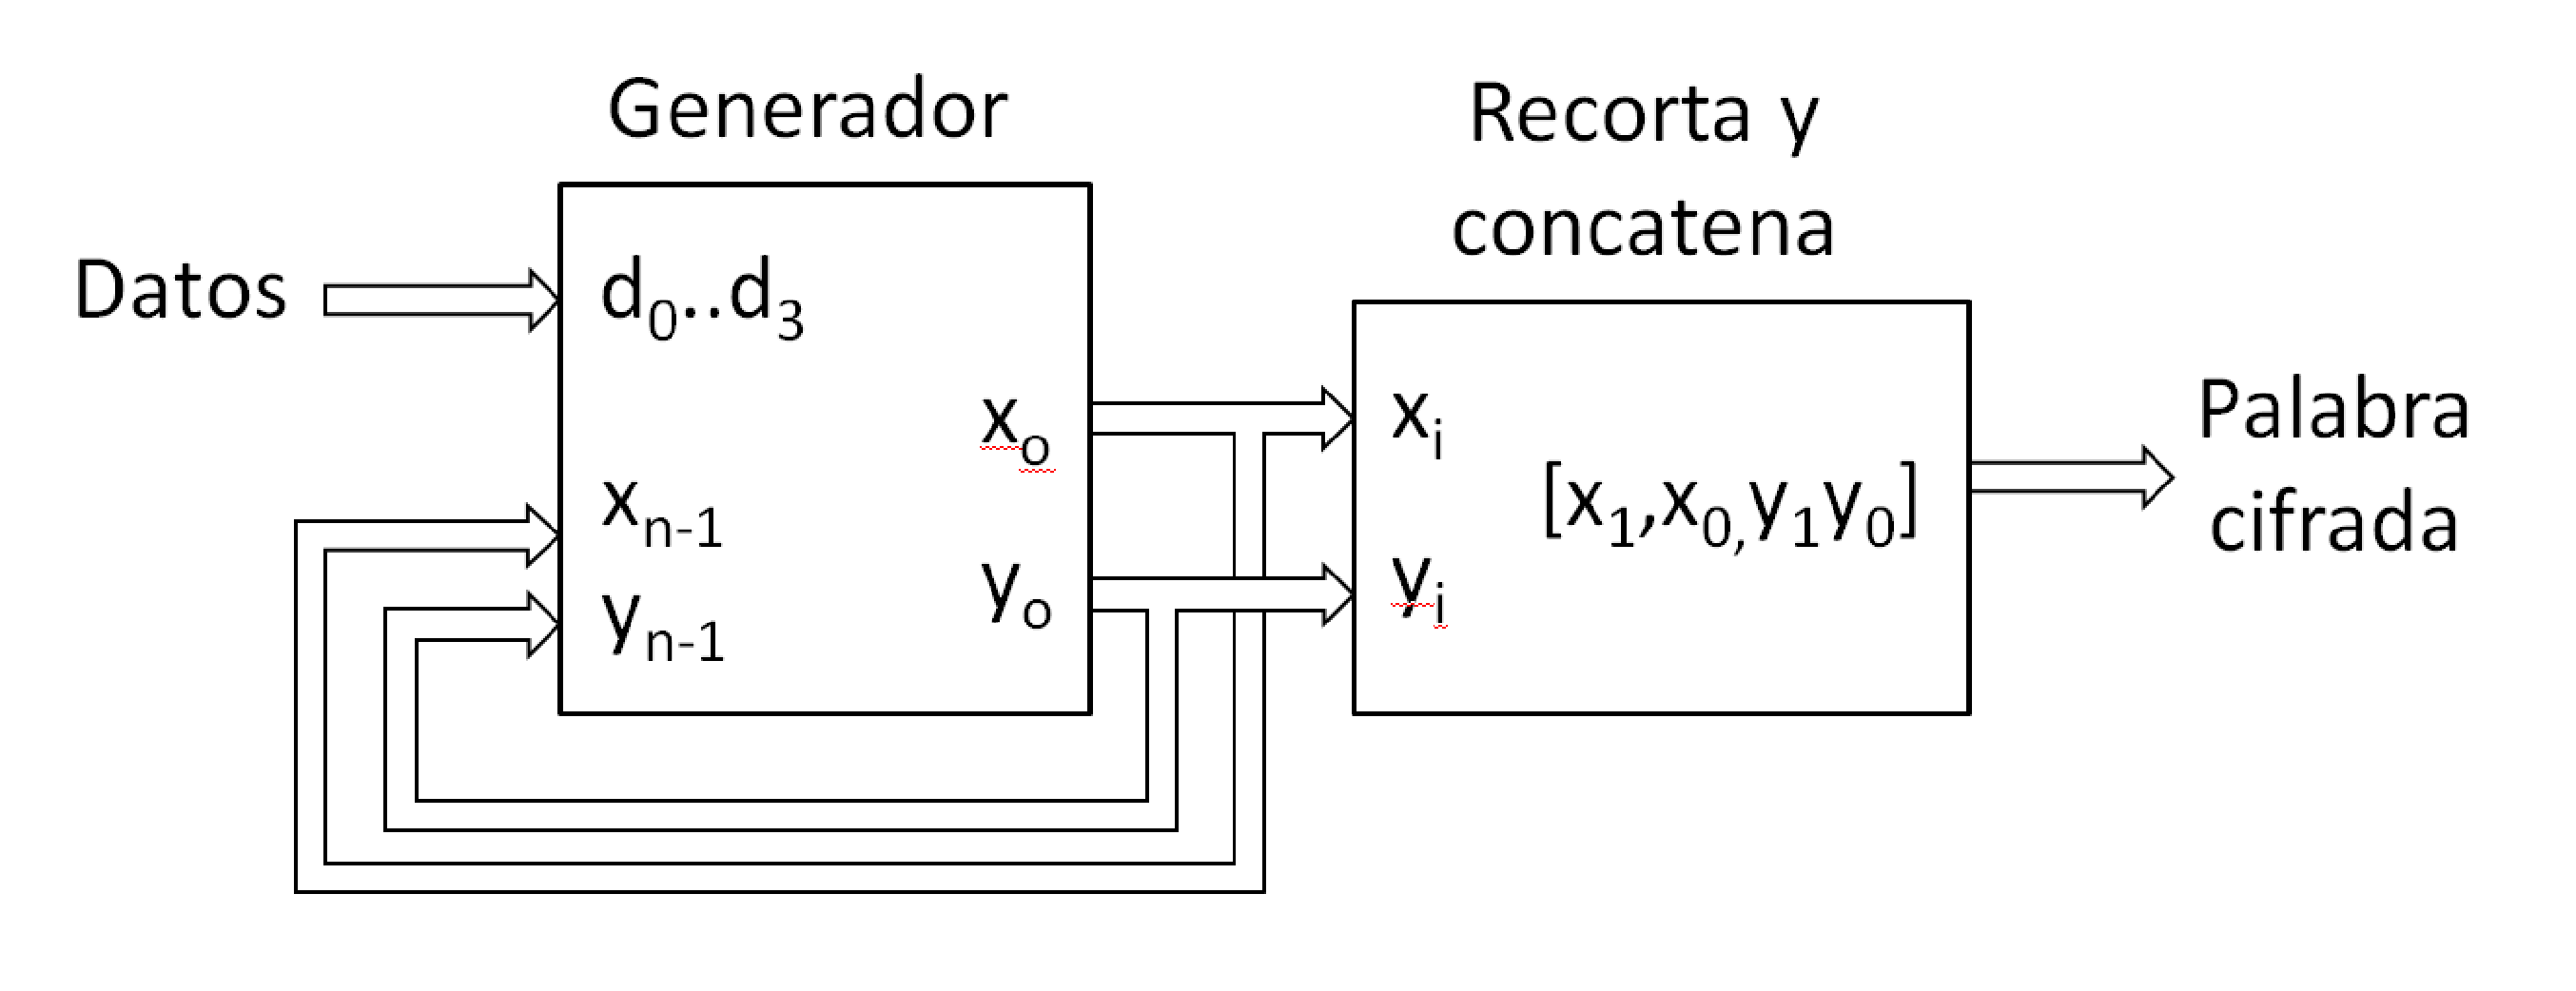
\includegraphics[width=0.8\columnwidth]{Fig2.pdf}\\
    \caption{Codificador.}\label{fig:codificador}
\end{figure}

\subsubsection{Decodificador}


Un segundo circuito generador de atractores funciona en el decodificador generando las $16$ palabras posibles para la próxima iteración. Luego, se ingresan todas estas posibles palabras
cifradas junto con la que se desea decodificar a un comparador que aplica una XOR a la palabra ingresada contra todas las palabras posibles generadas localmente para decodificarla. La
salida de este circuito es la palabra decodificada (Fig. \ref{fig:decodificador}).

\begin{figure}\
    \centering
    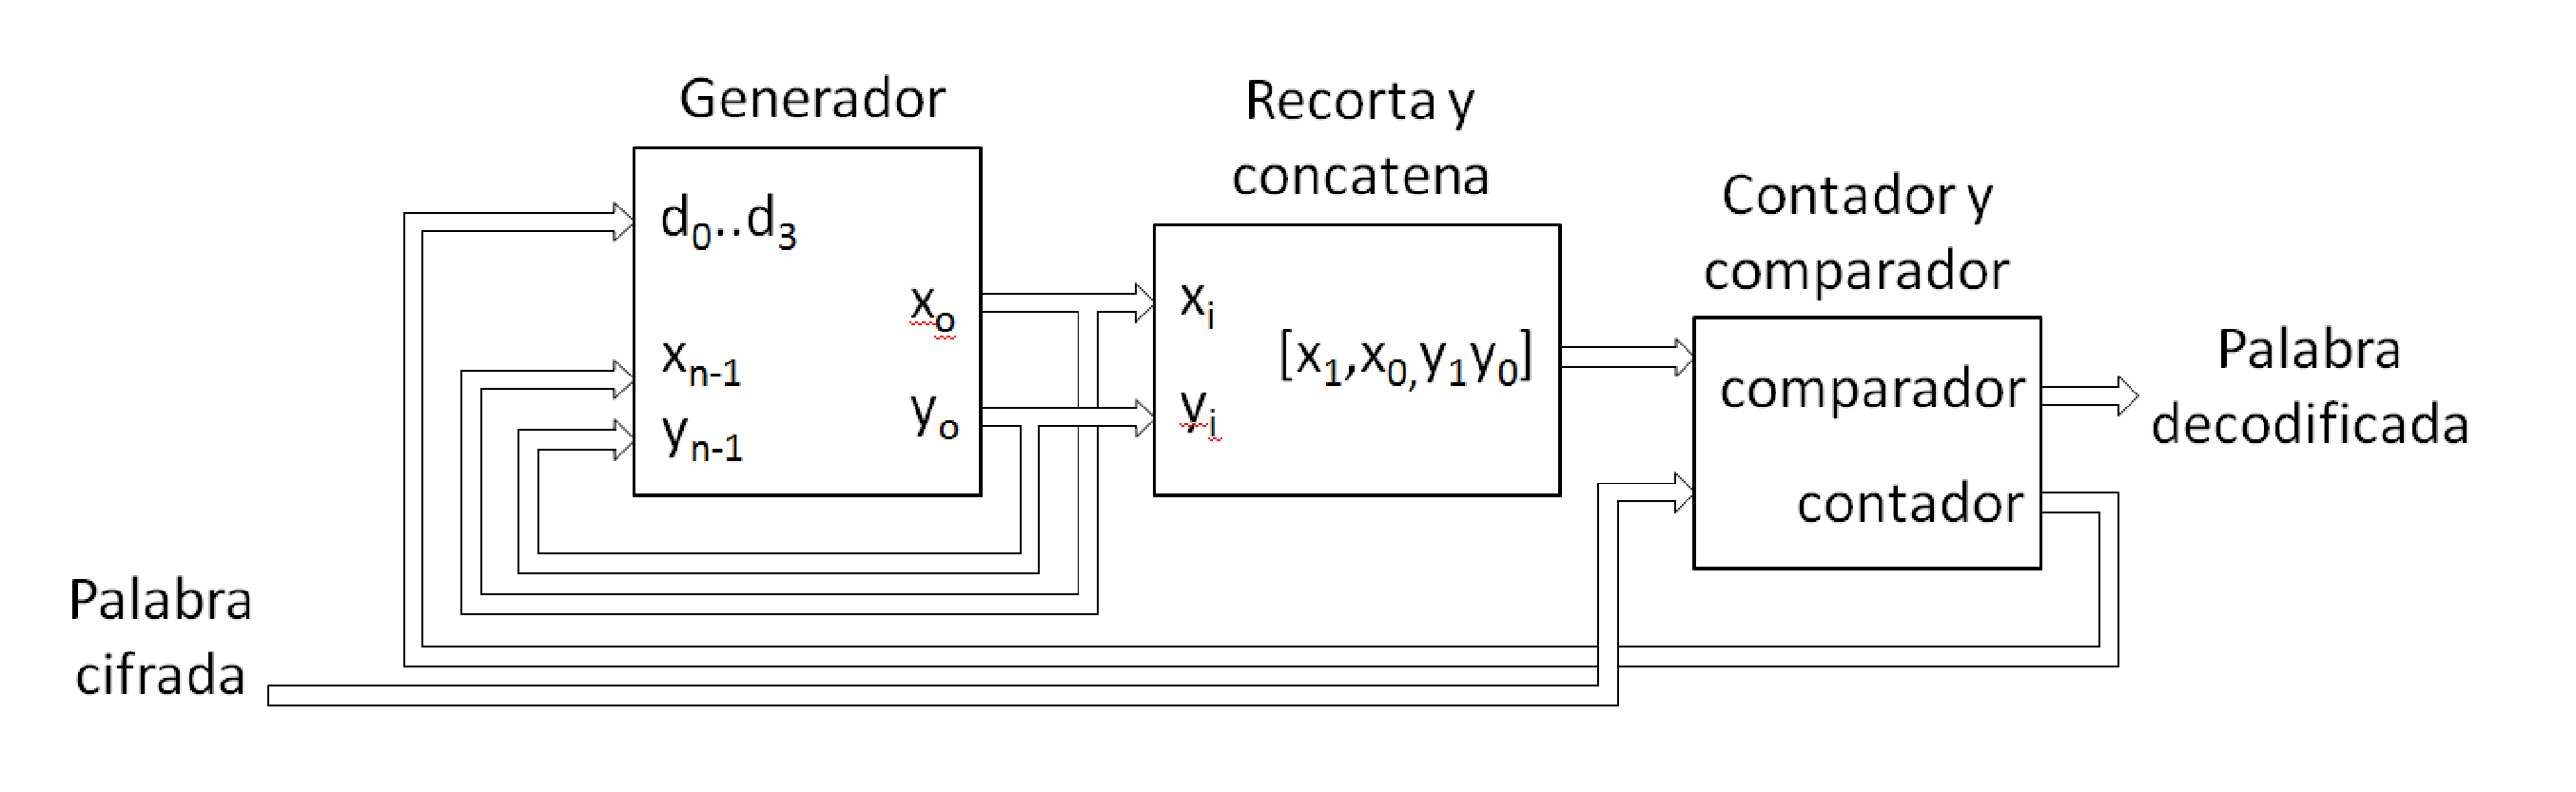
\includegraphics[width=0.8\columnwidth]{Fig3.pdf}\\
    \caption{Decodificador.}\label{fig:decodificador}
\end{figure}

\subsection{Resultados}
Se realizó un primer esquema del diseño mediante la herramienta
Quartus II v8.0 de ALTERA, para implementar el sistema en una FPGA \emph{Altera Cyclone III EP3C120}

Se obtuvieron resultados preliminares de simulaciones realizadas
mediante el programa Matlab y mediante simulaciones con el
programa Quartus de Altera, estas últimas tienen en cuenta el
empelo de la precisión finita elegida para representar los
valores.

En la Fig. \ref{senal} se pueden ver las salidas del bloque
generador para una transmisión de los datos
[1,2,3,2,3,3,1,3,1,3,1]. En este caso se mantiene el dato a enviar
durante $100$ ciclos con el objetivo de que sea visible en la
figura, en el sistema real cada oscilador codifica una palabra de
información en cada iteración. Aqui puede observarse que el
sistema cambia el atractor generado según los coeficientes que
dependen de la entrada de información a transmitir.

En cuanto al análisis de performance que presenta el sistema se
deben tener en cuenta dos aspectos:

\begin{itemize}
    \item
        La distancia mínima de la modulación codificada resultante. Esta  es
        usualmente empleada para proveer un límite de error en la región
        de piso.
    \item
        Una descripción precisa de la tasa binaria de error
        del sistema o BER (en inglés, Bit Error Rate) también es un
        parámetro muy importante, ya que da una estimación del
        comportamiento que presentara el código.
\end{itemize}


\begin{figure}
    \centering
    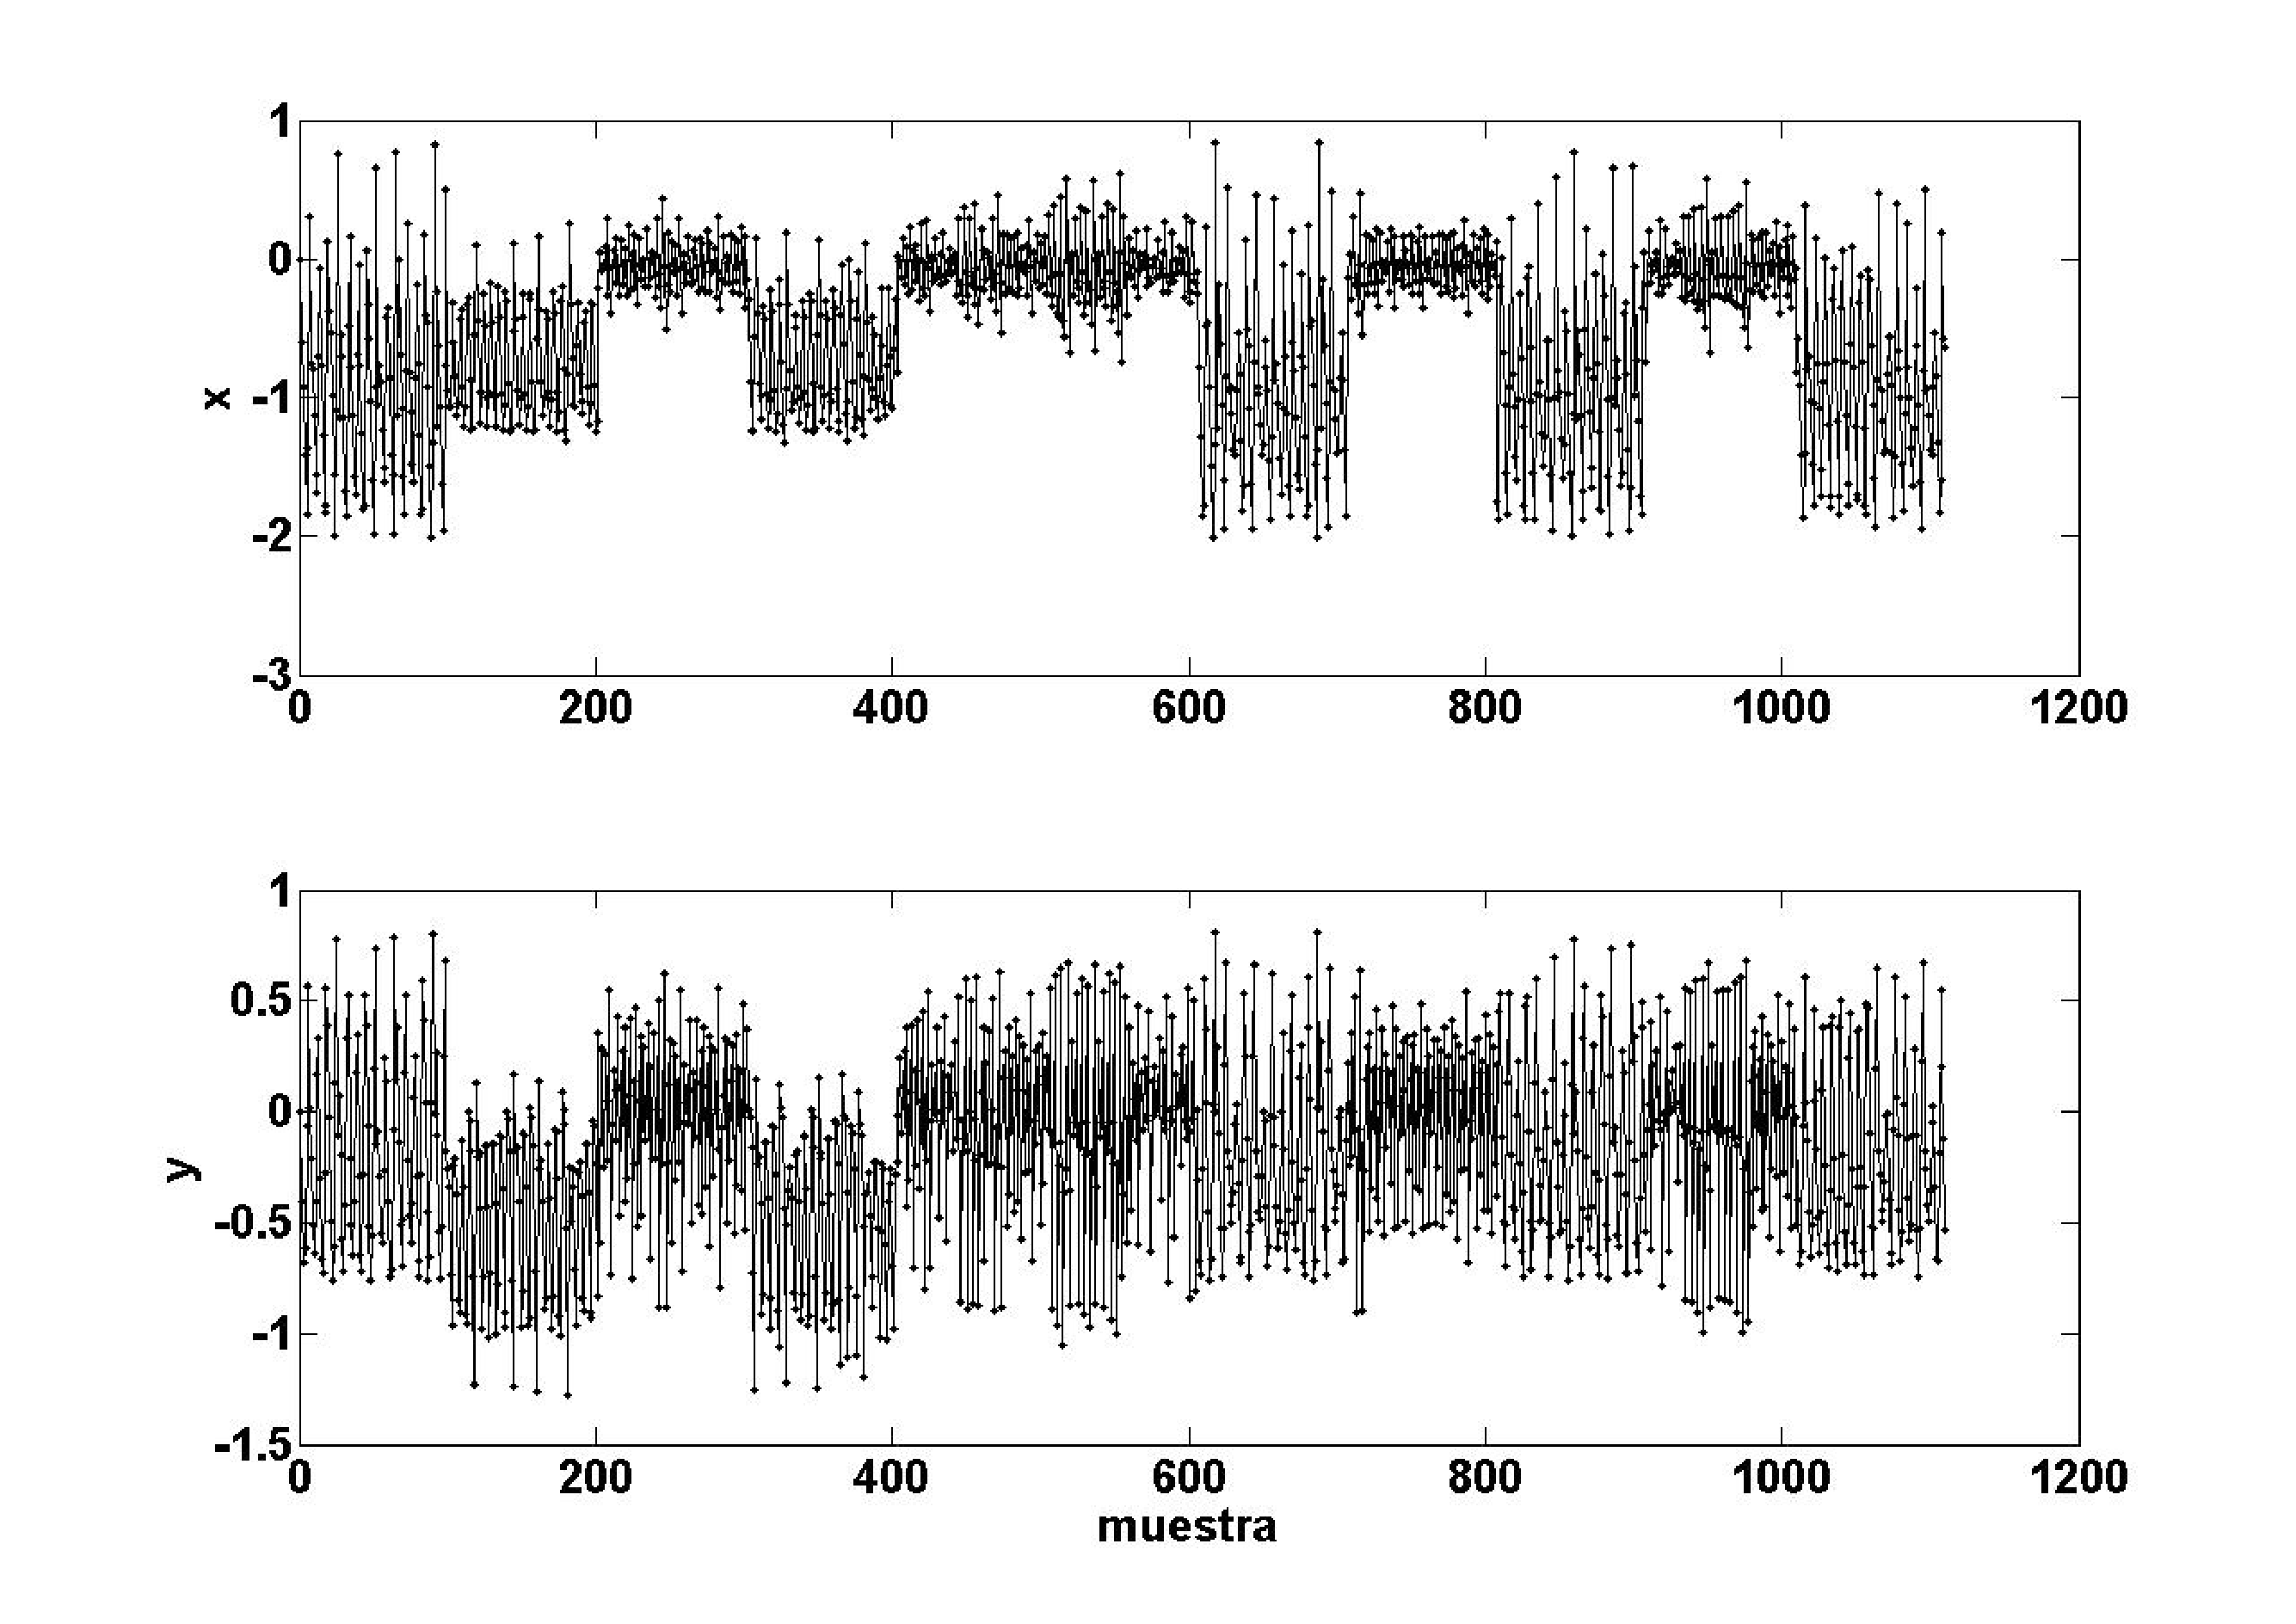
\includegraphics[width=1\columnwidth]{senalent.pdf}\\
    \caption{Señales a transmitir.}\label{senal}
\end{figure}

%\bibliography{xbibWEBjun2012_ingles}

%%%%%%%%%%%%%%%%%%%%%%%%%%%%%%%%%%%%%%%%%%%%%%%%%%%%%%%%%%%%%%%%%%%%%%%%%%%%%%%%%%%%%%%%%%%%

\section{Codificación variable en el tiempo empleando mapa caótico (póster CASE2012)}

Los posters no se si agregarlos o distribuir la información entre los demás capítulos.

En el diseño de un sistema de comunicaciones de datos inalámbrico tanto la confiabilidad de la
transmisión como el nivel de privacía son objetivos a cumplir. Han surgido últimamente técnicas de
codificación que permiten además de aumentar la confiabilidad de la transmisión frente al ruido adicionar
al sistema algún nivel de seguridad. En este trabajo se propone un esquema de codificación que cumple
con ambos objetivos. Este sistema se basa en un mapa cuadrático bidimensional cuya salida presenta un
comportamiento caótico y distintos atractores dependiendo de los coeficientes que se empleen.
Codificar significa básicamente tomar las 2k palabras binarias de k bits que se pretende codificar, y
asignarlas a algunos de los 2n vectores de n bits. Esto se realiza como una función unívoca entre los 2k y
los 2n vectores. Siendo regularmente k < n existen más vectores de n bits que los que se tienen de k bits.
Tradicionalmente el subgrupo de 2n palabras código es fijo y la elección de los vectores de n bits se realiza
empleando la menor redundancia, y maximizando la distancia o separación entre las palabras. En este
trabajo la asignación de los vectores es variable ya que a cada una de las 2k palabras a transmitir se le
asigna un juego de coeficientes que genera salida caótica del mapa. Según la palabra a transmitir el
sistema generará una salida determinada por los coeficientes y el valor inicial, esta será la palabra código
correspondiente a la palabra a enviar. De esta forma, el subespacio de palabras código va cambiando a
medida que la transmisión evoluciona.


%%%%%%%%%%%%%%%%%%%%%%%%%%%%%%%%%%%%%%%%%%%%%%%%%%%%%%%%%%%%%%%%%%%%%%%%%%%%%%%%%%%%%%%%%%%%%%%%%%

\section{Estudio del Caos en Redes Neuronales Discretas para su Implementación en Hardware (Informe Inteligencia computacional, Poster CASE2014)}

Este es bastante largo y completo, pero perdí todos los archivos junto con el disco, tengo el pdf a partir del cual voy a tener que armar el latex de nuevo.

Dentro de los sistemas complejos se encuentran los cóticos, éstos se caracterizan por tener
propiedades estocásticas similares a los de los sistemas aleatorios (en algunos casos mejores),
por ser muy sensibles a las condiciones iniciales y por ser impredecibles a mediano plazo a
pesar de contar con las ecuaciones que describen el sistema. Numerosos trabajos describen el
comportamiento caótico en redes neuronales, este trabajo presenta una detallada descripción
técnica de un caso de estudio.


%%%%%%%%%%%%%%%%%%%%%%%%%%%%%%%%%%%%%%%%%%%%%%%%%%%%%%%%%%%%%%%%%%%%%%%%%%%%%%%%%%%%%%%%%%%%

\section{\emph{RO}-based \emph{PRNG}: \emph{FPGA} implementation and stochastic analysis}

\subsection{Introduction}

The jitter and phase noises present in ring oscillators, are not
convenient in several applications of \emph{RO}s, for example in the implementation of \emph{on-chip oscillators} to generate clocks in high-speed circuits\cite{Hajimiri1999,Mandal2010,Gupta2011}. However they are the source of randomness for \emph{RO}-based \emph{PRNG} \cite{Sunar2007,Wold2009}. Furthermore \emph{RO}s can be implemented in a full-digital circuit like Field Programmable Gate Arrays (\emph{FPGA}s) as they  basically are just a string of inverters.


In \cite{Sunar2007}, Sunar et al. presented a \emph{PRNG} using
stochastic jitter by combining several \emph{RO}s. They required a
post processing of the bit stream, based on resilient functions,
to mask imperfections in the entropy source and to increase
immunity against changes in environmental conditions. The entropy of the bit stream was used to
validate the results in \cite{Sunar2007}.


Wold et al. \cite{Wold2009} proposed an enhanced version with
better random characteristics and without a post processing. They only
added an extra D flip-flop at each ring output. The
effectiveness of their proposal was tested by means of test suites available
in the open literature \cite{NIST2000,marsaglia1995,NIST2000a}.

In this paper a detailed description of a very compact hardware implementation of the \emph{RO}-based \emph{PRNG} proposed in \cite{Wold2009} is done.
In order to validate the randomness of the noise sequences generated, two quantifiers derived from the information theory are used. They define a dual entropy plane $H_{BP}$ vs $H_{hist}$.
$H_{hist}$ is a measure of the first characteristic of a \emph{PRNG} pointed in the abstract, the equiprobability among all possible values. $H_{BP}$ is a measure of the second characteristic pointed in the abstract, the independence between consecutive values. This methodology was successful to evaluate randomizing
techniques applied to chaos-based \emph{PRNG} \cite{DeMicco2008}. A comparison with other options both physical and algorithmic, proposed in the literature is made showing that, in spite of their simplicity, \emph{RO}  are good candidates as \emph{PRNG}.

Organization of the paper is as follows: section \ref{sec:hardware} describes the
hardware implementation of the \emph{RO}s mapped in
\emph{FPGA} Cyclone III. Section \ref{sec:method} shows how the normalized entropies are
determined (to keep this paper short we do not detail already
published results); \ref{sec:results} presents the
results obtained for different configurations of the same
\emph{PRNG}s proposed in \cite{Wold2009}, and the statistical comparison with other utilized \emph{PPRNG}s.
Finally we present our conclusions in Sec. \ref{sec:conclusions}.


\subsection{Hardware implementation.}

The implemented \emph{PRNG}'s consist of  several \emph{RO}s
with their outputs XORed together and sampled by a \emph{D} flip flop,
The flip flop latches the output at a selected frequency (here $100$MHz)\cite{Wold2009}.
The physical implementation is made on \emph{ALTERA}$^{\copyright}$  \emph{Cyclone} III \emph{EP3C120}
development kit with a \emph{EP3C120F780C7N} \emph{FPGA}. The design is made with \emph{Quartus}$^{\copyright}$  II 13.1 software.

\subsubsection{Chip Overview.}

\emph{FPGA}s consist of a large number of logic array blocks (\emph{LAB}s), with groups of logic elements (\emph{LE}s) for implementing sequential as well as
combinatorial circuits. In the \emph{Cyclone} III family architecture
each \emph{LAB} contains $16$ \emph{LE}s.
Basically, each \emph{LE} is a Flip Flop (\emph{FF}) with a
four-input look-up table (\emph{LUT})  (see Fig. \ref{fig:LE}). Each
\emph{LUT} can implement any function of
four variables. The \emph{FF} and the \emph{LUT} can be used together or independently, \cite{Altera}.

%=========================================
 % FIGURA
\begin{figure}
\begin{center}
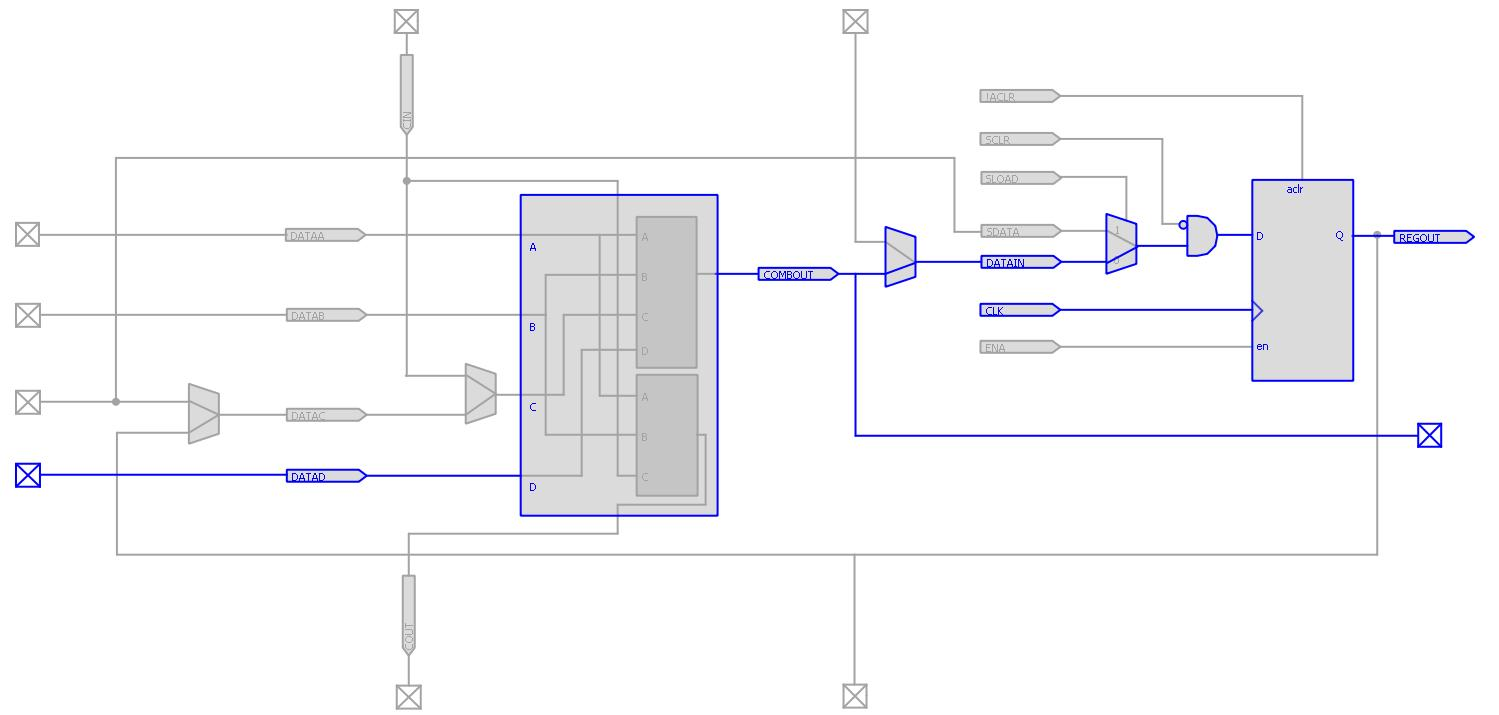
\includegraphics[ width=0.5\textwidth]{NOTenLEmasFF}
\caption{\emph{LE} implementing an inverter and a Flip Flop, Chip Planner
view.} \label{fig:LE}
\end{center}
\end{figure}
%=========================================

Usually, the logic synthesis software assigns \emph{LE}'s
resources without the designer intervention. But in the design of
\emph{RO}-based \emph{PRNG}s it is necessary to control the exact location of
each individual component for two reasons: 1) to avoid the
simplification of the inverters performed by the synthesis tool; 2) to locate
each \emph{RO} in the desired place. In \emph{Altera} the use of low-level primitives enables one to
control the hardware implementation for each \emph{cone of logic} \cite{LowLevel}. Consequently
low-level primitives and assignments are employed inside the \emph{HDL} (hardware description language) code employed in our design.

Strings of \emph{RO}s can be programmed on the chip by
instantiating the \emph{LUT}s as inverters.
In the case of \emph{RO}s it is necessary to prevent the \emph{Quartus} II synthesis engine to merge two \emph{NOT} gates in series, by using a primitive called \emph{LCELL}.
 A \emph{LCELL} always consumes one logic cell and it is not
removed from the project during logic synthesis.

These primitives allow one to break up the design into manageable parts. Each cone is as small as a \emph{LCELL} instantiation.
To create a \emph{RO}, \emph{LCELL}s are programmed as inverter-buffers. Figs. \ref{fig:RTL1ring} and \ref{fig:postMap1ring} show how this primitive is implemented by the Quartus II compiler.

\begin{figure*}
\begin{center}
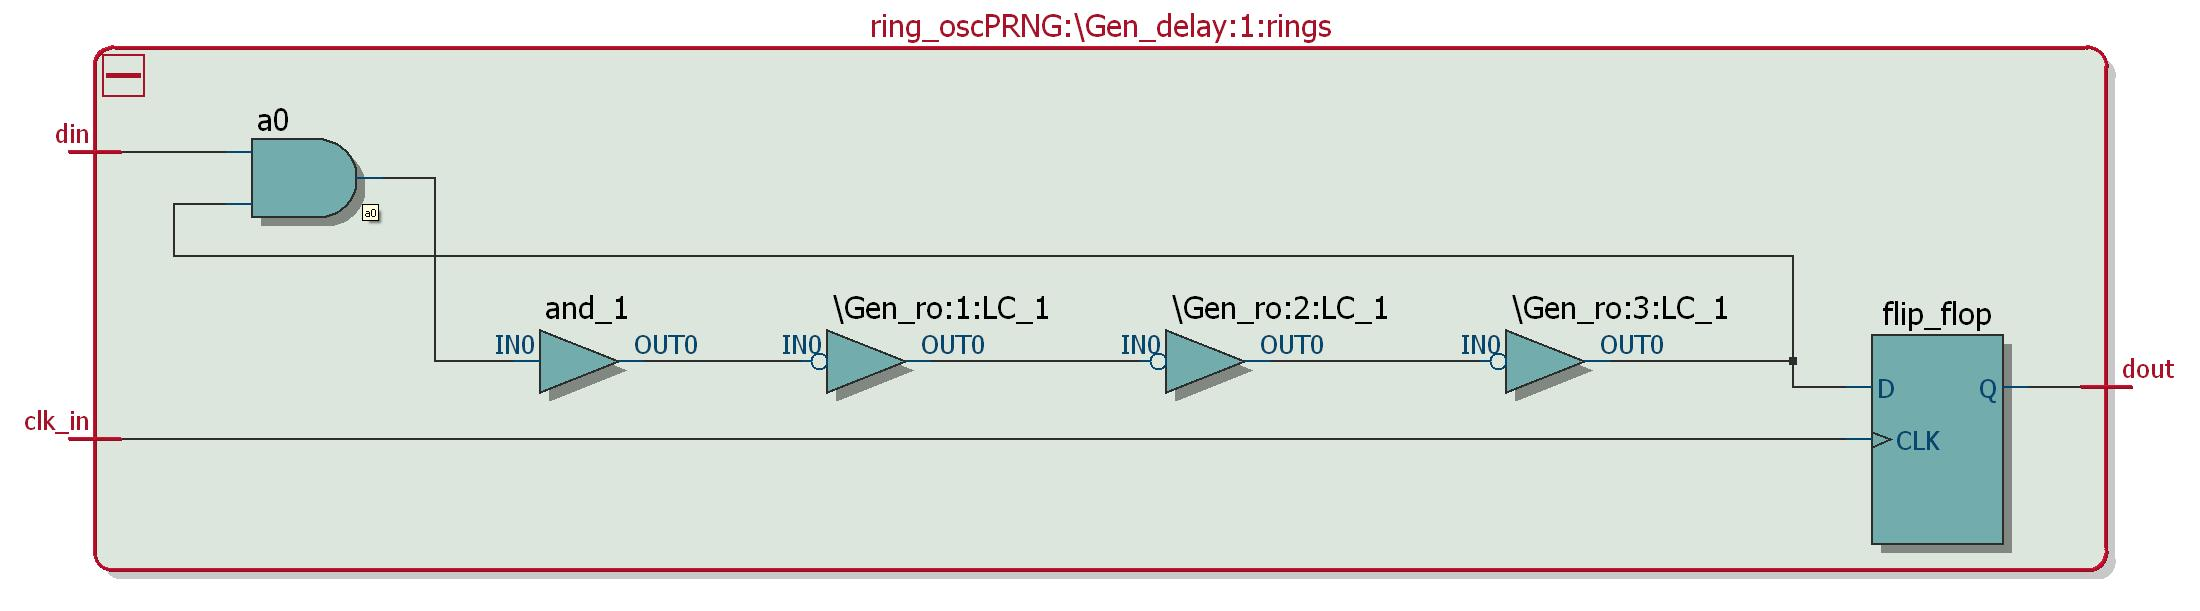
\includegraphics[ width=0.7\textwidth]{RTL_view_1ring}
\caption{RTL view one ring with $3$ inverters.}
\label{fig:RTL1ring}
\end{center}
\end{figure*}

%=========================================
 % FIGURA
\begin{figure*}
\begin{center}
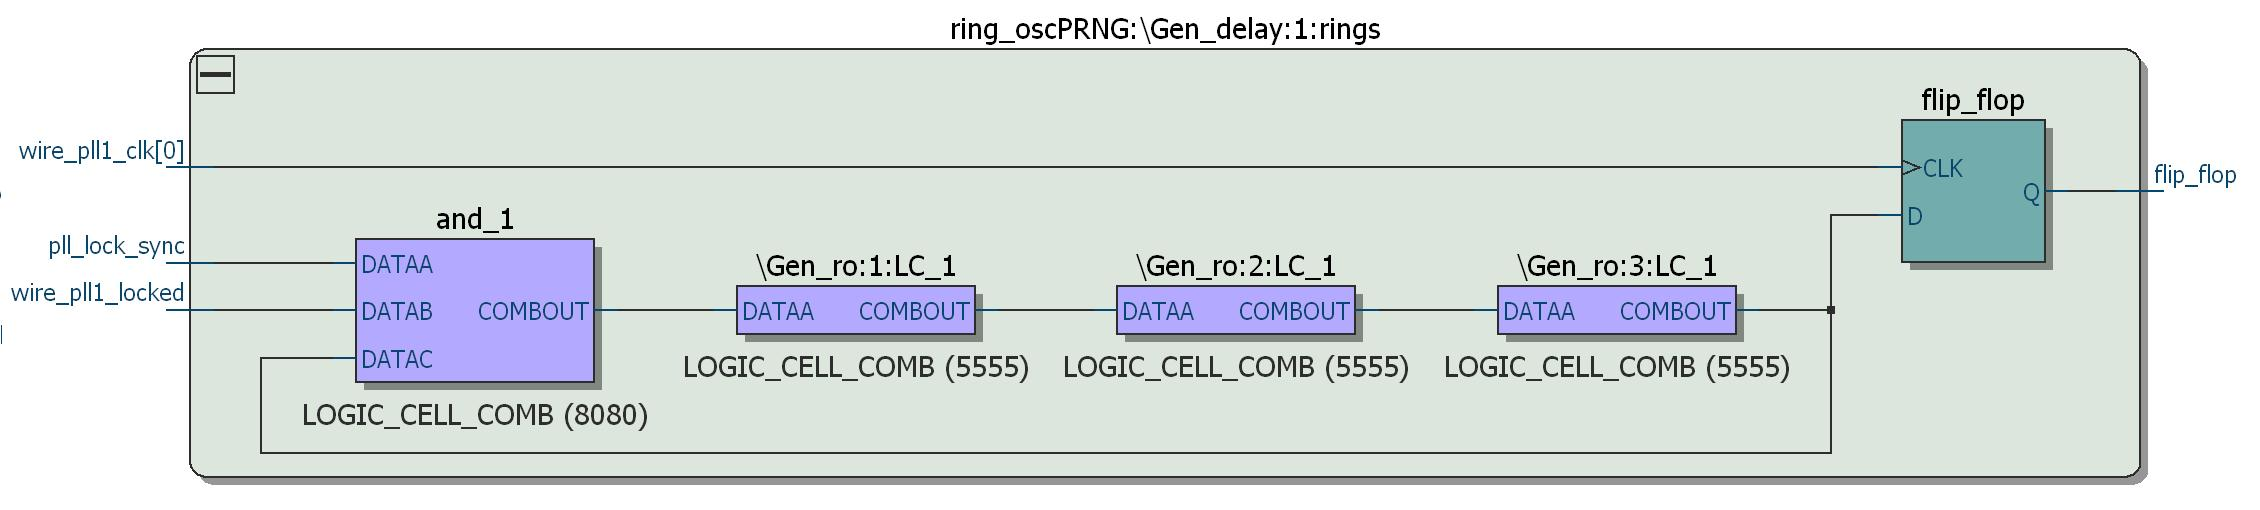
\includegraphics[ width=0.7\textwidth]{tech_map_viewer_post_mapping}
\caption{Technology map viewer (post mapping), one ring with $3$
inverters.} \label{fig:postMap1ring}
\end{center}
\end{figure*}
%=========================================

Furthermore, to avoid the synthesis tool to optimize removing the redundant buffers away,
the \empty{Ignore \emph{LCELL} Buffers} must be set in
\emph{OFF} in the \emph{More Analysis \& Synthesis
Settings} dialog box. Also \emph{Remove Redundant Logic Cells}
must be set to \emph{OFF}.

In order to place each \emph{RO} at a desired position, it
must be assigned to a previously defined \emph{LogicLock region}. In this way the \emph{fitter} will keep all the elements of each ring inside the same region,
\cite{LogicLockRegions}. The process of mapping all the elements to a particular location on the chip
(\emph{LogicLock} region) is achieved by the \emph{Assignment
Editor} tool, that also allows one to verify
that the placements are actually still there, after the  \emph{Synthesis} and \emph{Place \& Route} processes.

Fig. \ref{fig:fpgaplan} shows the $50$ \emph{LogicLock} regions used in this paper as they are
established in the die. One \emph{RO} is assigned to each region.
Regions are spread over the die for a future analysis of location importance. Each region has  $16$ \emph{LAB}s, to allow us to increase the number of inverters of each ring, an issue to be considered in future work.


%=========================================
 % FIGURA
\begin{figure*}
\begin{center}
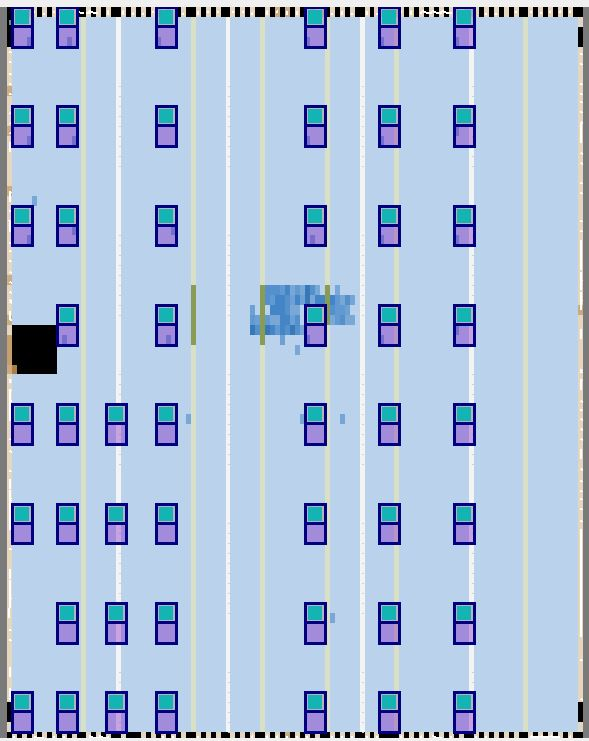
\includegraphics[ width=0.5\textwidth]{fpgaplan}
\caption{\emph{Chip Planner} view \emph{LogicLock} regions.}
\label{fig:fpgaplan}
\end{center}
\end{figure*}
%=========================================

 $3-$inverters, employed in a \emph{RO} and the \emph{FF} were all mapped onto a  \emph{LE} each, meaning that the block
utilization is $4$ of $16$ \emph{LE}s for any \emph{LAB}.


Fig. \ref{fig:LE} displays a single \emph{LE}, there an inverter is
implemented in the \emph{LUT} and it can be seen the exact
\emph{LUT} input that is used. Also the output \emph{FF} of
the ring is mapped there.


There are many factors that determine the frequency of each
\emph{RO}, and contributes to the unpredictability of the output:
\begin{enumerate}
\item Placement within the \emph{LAB}: different placements between rings could result in timing differences.
\item Connections: even having exactly
identical placement of the \emph{LUT}s with respect to each other
in a given ring, it is not possible to have exactly the same
\emph{routing resource usage} in the connections. A small difference in
\emph{routing resource usage} could affect the ring delay.
\item Input selection:  the \emph{fitter} will choose which
\emph{LUT} input is utilized during the routing stage. But the delay through the \emph{LUT}
depends on which of the four inputs is used and consequently the rings could
also have different delays.
\item Neighborhood: even if the design locks down all the placement and routing of a
section  and everything is
physically locked, the timing can change by a few picoseconds
depending on what is placed and routed around the ring.\end{enumerate}
%
In Fig. \ref{fig:RTL3rings} (RTL view) it is shown a \emph{PRNG} using $3$ \emph{RO}s
followed by a XOR gate.

% FIGURA
\begin{figure}
\begin{center}
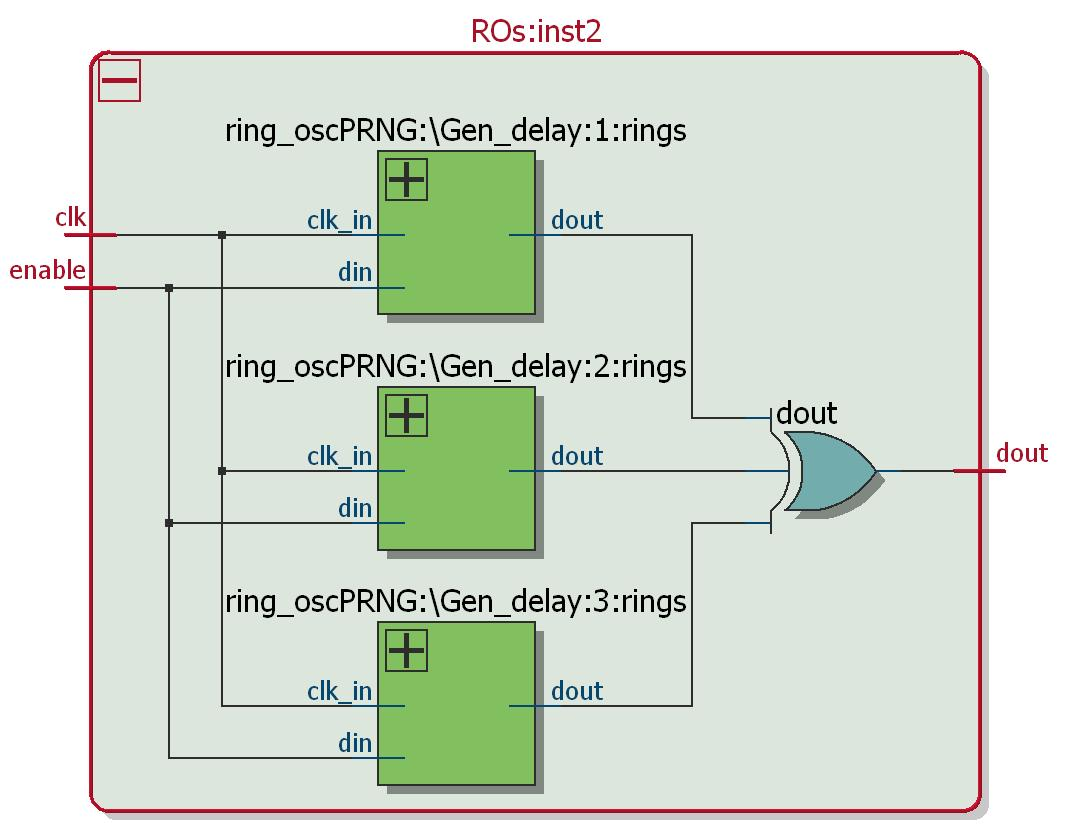
\includegraphics[ width=0.5\textwidth]{RTL_view_3ROs}
\caption{\emph{RTL} view of \emph{PRNG} with $3$ \emph{RO}s.}
\label{fig:RTL3rings}
\end{center}
\end{figure}

%=========================================

Finally, Table \ref{compilation} shows the compilation report of the \emph{PRNG}  using $15$ \emph{RO}s each with $3$ inverters.


%=========================================
\begin{table}
\begin{center}
\begin{tabular}{| l | c  c | }
 \hline
 
\footnotesize{Total logic elements} & $847/119,088$ & $ ( < 1 \%)$\\

 \hline
 
\footnotesize{Total combinational functions} &  $629/119,088$ & $( < 1 \%)$ \\

 \hline
 
\footnotesize{Dedicated logic registers} & $617/119,088$ & $( < 1 \%)$ \\

 \hline
 
\footnotesize{Total registers} &  $617$ &   \\

 \hline
 
\footnotesize{Total memory bits} &  $131,072/3,981,312$ & $( 3 \%)$ \\

 \hline
 
\end{tabular}
\end{center}
\caption{Compilation Report, \emph{RO}-based \emph{PRNG} using $15$ \emph{RO}s and $3$ inverters each.}
\label{compilation}

\end{table}




%==========================================



\subsection{Quantifiers}
\label{sec:method}
Let $X=\{x_i, i=1,...,N\}$ be a length $N$  output of a given
symbolic source with alphabet $\mathcal{A}=\{a_i,i=1,...M\}$. Each
element of $X$ is  $x_i \in \mathcal{A}$. In the case of \emph{RO}
the alphabet is binary consisting of two symbols
$\mathcal{A}=\{0,1\}$. The output is converted into words of $n$
elements. In our case $n=6$. It means we work with a time series
$Y=\{y_i,i=1,...K$ with $K=N/6\}$  of natural numbers $y_i\in [0,2^6-1]$.

The obvious \emph{PDF} (probability density function) to characterize $Y$ is the normalized histogram of the $K$
words $Y$; let us call it  $PDF_{hist}$. Its normalized Shannon
entropy $H_{hist}$ is given by:
\begin{equation}
\label{eq:entropia}
H_{hist}=\frac{\sum_{i=1}^{K}{p_i~log~p_i}}{logK}
\end{equation}

We call this \emph{PDF}  \emph{non-causal} because it does not
change if we permute the time order of the words, and consequently
can not detect any causal connection between consecutive words. The normalized entropy
$H_{hist}$ quantifies the equiprobability of the words among all
possible values. For a \emph{PRNG} its ideal value is
$H_{hist}=1$.

To quantify statistical independence between consecutive words we
use a \emph{causal} \emph{PDF}, proposed by Bandt \& Pompe
\cite{Pompe2002}. This \emph{PDF} is obtained by assigning
ordering patterns to overlapped segments, of length $D$, of the
time series trajectory. The process is as follows: 1) group $D$
consecutive words $\{y_i,y_{i+1},...,y_{i+D}\}$ (let us stress that in our case each
$y_i$ is a natural number $\in[0,63]$). The ordering of the $D$
values inside each group is compared with the order of numbers
$\{1,2,...,D\}$. There exist $D!$ possible permutations of $D$ elements.
Each permutation is called an \emph{ordering pattern}
\cite{Amigo2006} and is labelled with a permutation number
$\pi=1,...,D!$. The normalized histogram of $\pi_i$'s is called
the Bandt \& Pompe \emph{PDF}, $PDF_{BP}$. The normalized Shannon entropy of
this $PDF_{BP}$ is $H_{BP}$ where the subscript $BP$ means ``Bandt
and Pompe".

In case two values of $y_i$ inside the same group are identical,
it is considered that the first one is lower than the last one in
order to obtain an unique result. For \emph{PRNG}s this procedure
does not produce significant changes in  $PDF_{BP}$.

The  Bandt \& Pompe procedure has the advantages of being: 1) simpler and
fast to calculate than block entropies, 2)
robust in presence of noise, and 3) invariant to lineal
monotonous transformations. It is applicable not only to
\emph{PRNG}s but also to any weak stationary process (it means for $k=D$,
the probability that $x_t < x_{t+k}$ does not depend on the
particular $t$ \cite{Pompe2002}). The causality property of $PDF_{BP}$
makes the quantifiers based on this \emph{PDF} to discriminate
between deterministic and stochastic systems \cite{Rosso2007B}.

Bandt and Pompe suggested $3\leq D \leq7$. $D=6$ is adopted
in this work.

A full discussion about the convenience of using different quantifiers
to measure a given \emph{PDF}is out of the scope of this work.
Nevertheless reliable bibliographic sources
do exist \cite{Wackerbauer1994,Lopez1995,Rosso2007A,DeMicco2008,Rosso2009,Martin2006,Rosso2012}.

In this paper we adopt plane $H_{BP}$ vs $H_{hist}$ \cite{DeMicco2008}  to represent each \emph{PRNG}. A higher
value in any of the entropies, $H_{BP}$ and $H_{hist}$, implies an
increase in the uniformity of the involved \emph{PDF}'s. The point
$(1,1)$ represents the ideal point for a \emph{PRNG} with uniform histogram and
uniform distribution of ordering patterns.

\subsection{Results}
\label{sec:results}
%

The  \emph{Embedded Logic Analyzer} tool is utilized for collecting the random sequences generated.
It constitutes a \emph{system-level debugging tool}, provided by $Altera$  \cite{QUARTUS}, that captures and storages the real-time signal behavior and allows one to observe interactions between hardware and software in system designs. After acquiring
the data and  save them into a \emph{SignalTap} II file, they can be
analyzed or viewed as a waveform. With this procedure nor extra jitter neither distortion are introduced in the measured signal from the data acquisition chain.


In the case of \emph{RO} based \emph{PRNG}
data files with $917504$ bits each were generated for each \emph{RO} based \emph{PRNG}.
We consider sets of $N_{RO}$ rings, each with $3$ inverters; $N_{RO}=2$, $3$, $4$, $5$, $6$, $7$, $15$, $25$ and $50$.

Data from $SignalTap$ were  processed using \emph{Matlab}$^\copyright$. Binary data were grouped in $6$-bits words without
superposition, so files with $152917$ data each were generated. Quantifiers described in section \ref{sec:method} were calculated
for all generated files.

We also evaluated other known noises generators to compare their quality with that of  the \emph{RO}-based \emph{PRNG}.
The noises analyzed are:


\begin{itemize}
  \item Mersenne Twister pseudo-random number generator, \cite{Matsumoto1998}.
  \item Two algorithms employed for generate random data by Matlab (Multiplicative Congruential method) \cite{Matlab} and Excel \cite{McLeod1985}.
  \item Two \emph{physical noises}: radioactive decay noise \cite{Walker2001} and atmospheric noise \cite{Haahr}.
  Data files for these noises are available from the referred \emph{websites}.
  \item Two chaotic map $M^1$ and their iterated versions $M^2$ to $M^8$ \cite{DeMicco2008} for the logistic map (\emph{LOGISTIC}) and the \emph{three way Bernoulli map} (\emph{TWBM}).
\end{itemize}

Fig. \ref{fig:HBPvsHhis_all} shows the results in the dual entropy plane $H_{BP}$ vs $H_{hist}$ for all these noises.
It can be seen that the \emph{physical noises}, the algorithmic \emph{Mersenne Twister}, and the \emph{PRNG}s used in \emph{Matlab} $^\copyright$(\emph{rand} function) and \emph{Excel}$^\copyright$ (\emph{RAND} function), have the  maximum value for $H_{BP}$, indicating that all the ordering patterns appear almost the same number of times. However these five noises present very different behavior with respect the $H_{hist}$ quantifier. The \emph{radioactive decay} is the worst, with a value of $H_{hist}$ about $0.5$ indicating that this sequence does not exhibit all possible values in the same proportion. In Fig. \ref{fig:HBPvsHhis_all} the numbers next to each marker for the chaotic sequences, indicate the number of iteration. The iterated maps have higher $H_{BP}$ because of their mixing property \cite{DeMicco2008}.


 % FIGURA
\begin{figure*}
\begin{center}
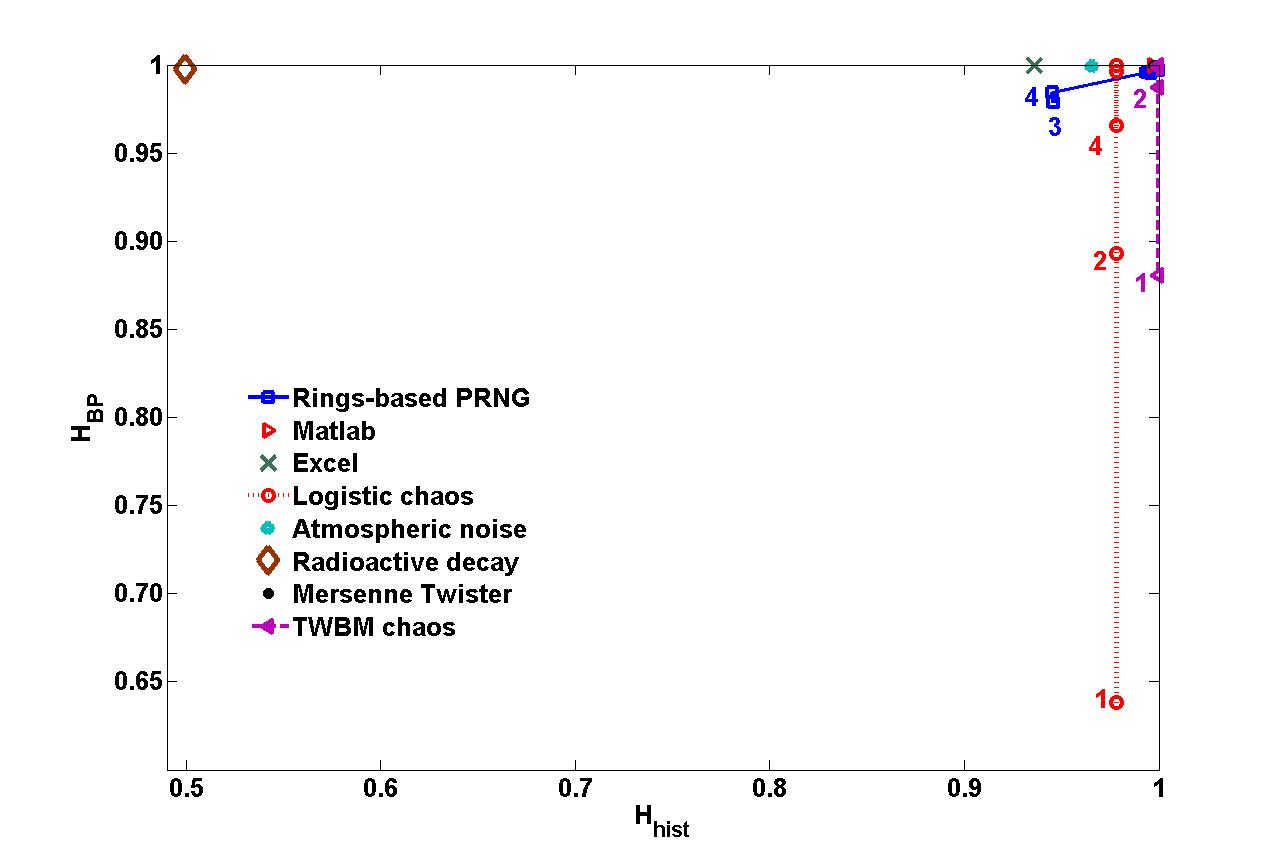
\includegraphics[ width=0.8\textwidth]{HhistvsHBP_t}
\caption{$H_{BP}$ vs $H_{hist}$ plane for several noises, numbers next to each square indicate the quantity of \emph{RO}s
used in the \emph{RO} based \emph{PRNG}. Numbers next to each point in the  chaotic sequences labeled \emph{Logistic}
and \emph{TWBM} indicate the number of iteration of the chaotic map (see the text for details).}
\label{fig:HBPvsHhis_all}
\end{center}
\end{figure*}
%=========================================

In the case of the \emph{RO}-based \emph{PRNG} sequences, numbers next to each square indicate the quantity of \emph{RO}s employed in that \emph{PRNG} (let us stress that the number of inverters is fixed to $3$). The dual entropy plane shows that  an increase in the number of \emph{RO}s improves both $H_{BP}$ and $H_{hist}$.

Fig. \ref{HhistvsHBP_zoom} is a zoom of Fig. \ref{fig:HBPvsHhis_all}  around the ideal point $(1,1)$.


%=========================================
 % FIGURA
\begin{figure*}
\begin{center}
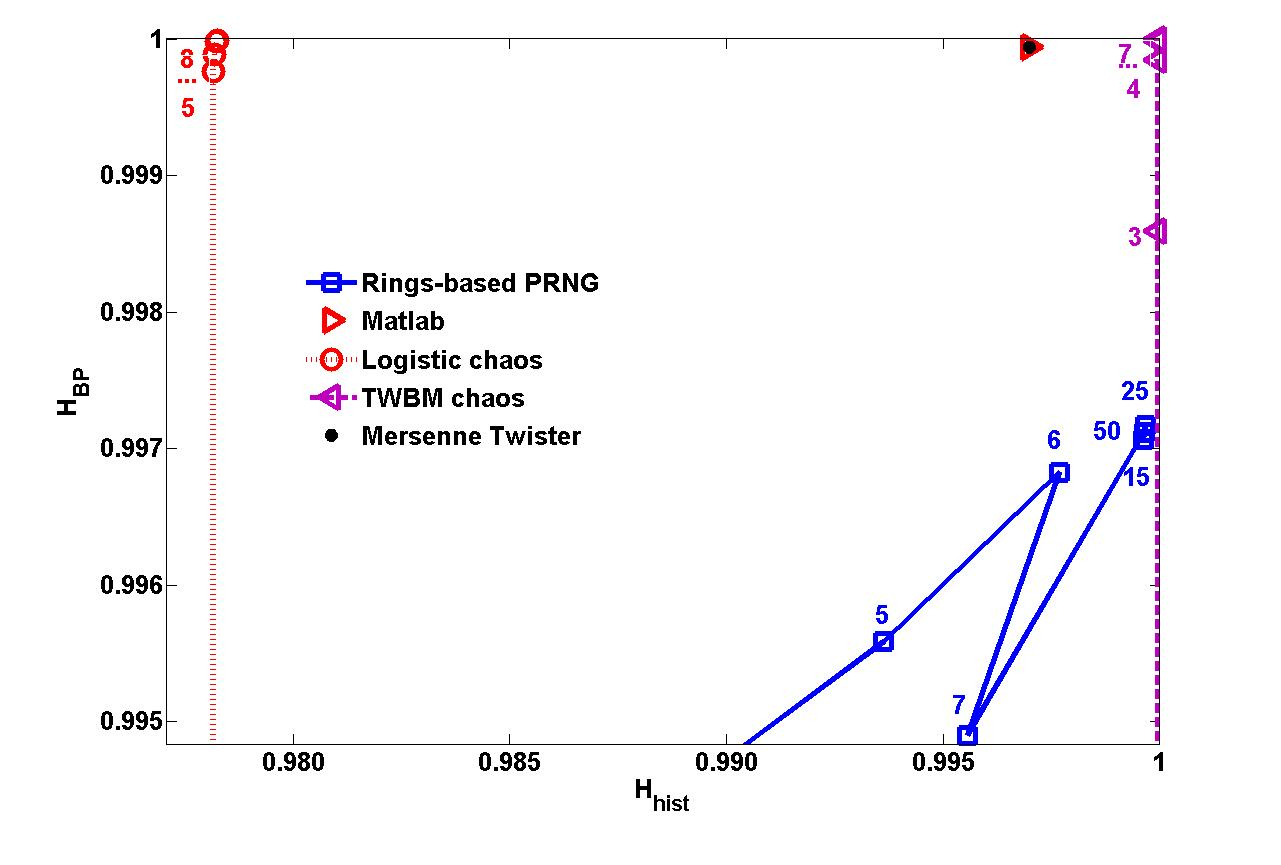
\includegraphics[ width=0.8\textwidth]{HhistvsHBP_z}
\caption{Zoom of Fig. \ref{fig:HBPvsHhis_all}  around the ideal point $(1,1)$ of the $H_{BP}$ vs $H_{hist}$ plane. Numbers next to each square indicate the number of \emph{RO}s used in that rings-based \emph{PRNG}. Numbers next to each point in the chaotic sequences indicate the number of iteration of the chaotic map.} \label{HhistvsHBP_zoom}
\end{center}
\end{figure*}
%=========================================

There, it is shown the evolution of the \emph{RO}-based \emph{PRNG} sequences when the quantity of \emph{RO}s increases from $5$ to $50$ (numbers next to each square). It can be seen that as the number of rings increases, data increase their mixture and also the histogram tends to be more uniform. So both properties are improved. Here a threshold in the number of rings can be determined, as the points saturate at about $(0.997,1)$, so this is the best \emph{PRNG} possible. Further, using more than $15$ \emph{RO}s presents no improvement.
As it was previously said, $H_{hist}$ quantifier detects the histogram variation of the sequence, and the $H_{BP}$ quantifier reflects the improvement in the mixing of data.
Finally, Mersenne Twister and Matlab sequences present identical value, ideal $H_{BP}$, and a high value of $H_{hist}$ nonetheless the histogram is not perfectly uniform (values are not equiprobable).

\subsection{Conclusions}
\label{sec:conclusions}
\emph{RO}-based \emph{PRNG} implemented here has demonstrated to satisfactorily meet the statistical properties desired by a \emph{PRNG}. They are comparable of other used \emph{PRNG}s and in some cases they are better. They employs few resources of the device and they are simply to implement in a digital platform.

It was demonstrated that for these architectures of \emph{PRNG} the quantity of
\emph{RO}s establishes \emph{PRNG}'s statistical properties. It was seen that
for $15$ \emph{RO}s both output's statistical properties, histogram
and mixing, were almost ideal, making unnecessary the increase of the number of rings.

The dual entropy plane proposed here has demonstrated to satisfactorily discern between the \emph{PRNG}'s two main desired properties, the equiprobability among all possible values and the statistical independence between consecutive values. Thus, it allows to clearly see what needs to be improved in a given sequence.



%\bibliographystyle{IEEEtran}
%\bibliography{xbibwebjulio2014_ingles,xbibMAXI_300314}  %


%%%%%%%%%%%%%%%%%%%%%%%%%%%%%%%%%%%%%%%%%%%%%%%%%%%%%%%%%%%%%%%%%%%%%%%%%%%%%%%%%%%%%%%%%%%%%%%%%

\section{Implementación de algoritmo genético para la búsqueda automática de caos en sistemas multiatractores (póster CASE2013)}

Se generó una lógica basada en algoritmos genéticos encargada de evolucionar los
parámetros del sistema de modo que cada generación tenga un comportamiento
caótico mejor que la anterior [3]. El target (fitness function), por lo tanto, es el MLE.
Para mayor claridad se separó el diagrama de flujo en dos partes, un diagrama principal
y una subrutina.
El sistema se inicializa en un conjunto de coeficientes llamado población inicial,
semilla o padre y se calcula su fitness function (Fp). Luego, se genera un incremento de
estos parámetros generando un hijo, que ingresa a la subrutina Evolution que lo
devuelve evolucionado y calcula su fitness function (Fc) para compararla con la de sus
padres. Las posibilidades son tres: el hijo es un padre de la siguiente generación
reemplazando al padre o no, o el hijo es descartado.
La subrutina Evolution es un algoritmo muy simple basado en mutaciones. Se
varían ligeramente los coeficientes del sistema (generando mutaciones) evaluando su
fitness function (Fm) buscando un máximo local.
